\section{Giới thiệu}

% 2 slide
% - Slide 1: Bài toán tô màu ảnh độ xám là gì, nói bài toán này là tạo sinh màu
% - Slide 2: Trong nhiều thập kỷ, ảnh đen trắng đã giữ vai trò quan trọng trong lưu trữ lịch sử, y khoa, giám sát và truyền thông. Tuy nhiên, việc khôi phục lại màu sắc thực tế cho các ảnh độ xám không chỉ mang ý nghĩa thẩm mỹ, mà còn đóng vai trò quan trọng trong việc hiểu ngữ nghĩa, phân tích nội dung và tăng cường trải nghiệm thị giác.

% Một số ứng dụng: lịch sử khuôn mặt, 
% - Slide 3: Ngoài ra còn ưng dụng trong lĩnh vực thiết kế nội thất hay trang phục
% - Slide 4: Đầu vào đầu điều kiện giúp bổ trợ cho quá trình tô màu (có hoặc không) nêu về cái input là kênh L và các loại khác
% - Slide 5: Thách thức
% - Slide 6: Mục tiêu

% - Slide 7: 3 mô hình có các kiến trúc phổ biến, nêu hạn chế --> xong nếu palltet học từ gốc tốn nhiều tài nguyên
% - Slide 8: ControlColor tô màu dựa trên controlnet nhưng lại sử dụng quá nhiều dạng dữ liệu học làm mô hình dễ mất tập trung và nhầm lẫn, tinh gọn lại chỉ sử dụng text và ảnh độ xám.

% - Slide 9: Control Net ban đầu có mạng tạo sinh đã được huấn luyện sẵn
% - Slide 10: Mục tiêu, khúc cuối phải nói về việc sử dụng phiên bản pretrain stable diffusion

% \begin{frame}{Vấn đề}
%     Người ta tìm cách tận dụng khả năng của các mô hình ngôn ngữ lớn tìm kiếm mã nguồn phù hợp để dùng trong kho dữ liệu có sẵn.

%     \vspace{0.3cm}
%      Tuy nhiên, các mô hình ngôn ngữ lớn (LLMs) được phát triển với mục đích chính là tạo sinh các token, việc áp dụng trực tiếp chúng cho truy xuất và tìm kiếm mã nguồn gặp hạn chế bởi sự giới hạn độ dài chuỗi đầu vào gây khó khăn cho tác vụ truy xuất quy mô lớn. 
     
%     \vspace{0.3cm}
%     Do đó, giải pháp gián tiếp cho bài toán này là dùng LLM để sinh ra mã nguồn mẫu và truy vấn dựa vào chúng (framework GAR).
% \end{frame}

\begin{frame}{Giới thiệu bài toán}
\begin{figure}
    \centering
     \includegraphics[width=0.7\linewidth]{Figures/mother-during-the-great-depression-1963.jpg}
\end{figure}
Tô màu ảnh độ xám là quá trình dự đoán các giá trị màu cho một ảnh độ xám, sao cho ảnh kết quả phù hợp nhất với nhu cầu sử dụng.

\end{frame}

\begin{frame}{Bối cảnh và động lực nghiên cứu}
\begin{figure}
    \centering
     \includegraphics[width=0.75\linewidth]{Figures/boicanh.png}
\end{figure}
Phục hồi ảnh lịch sử, ảnh chân dung, ảnh trắng đen lúc trước,...
\end{frame}

\begin{frame}{Bối cảnh và động lực nghiên cứu}
\begin{figure}
    \centering
     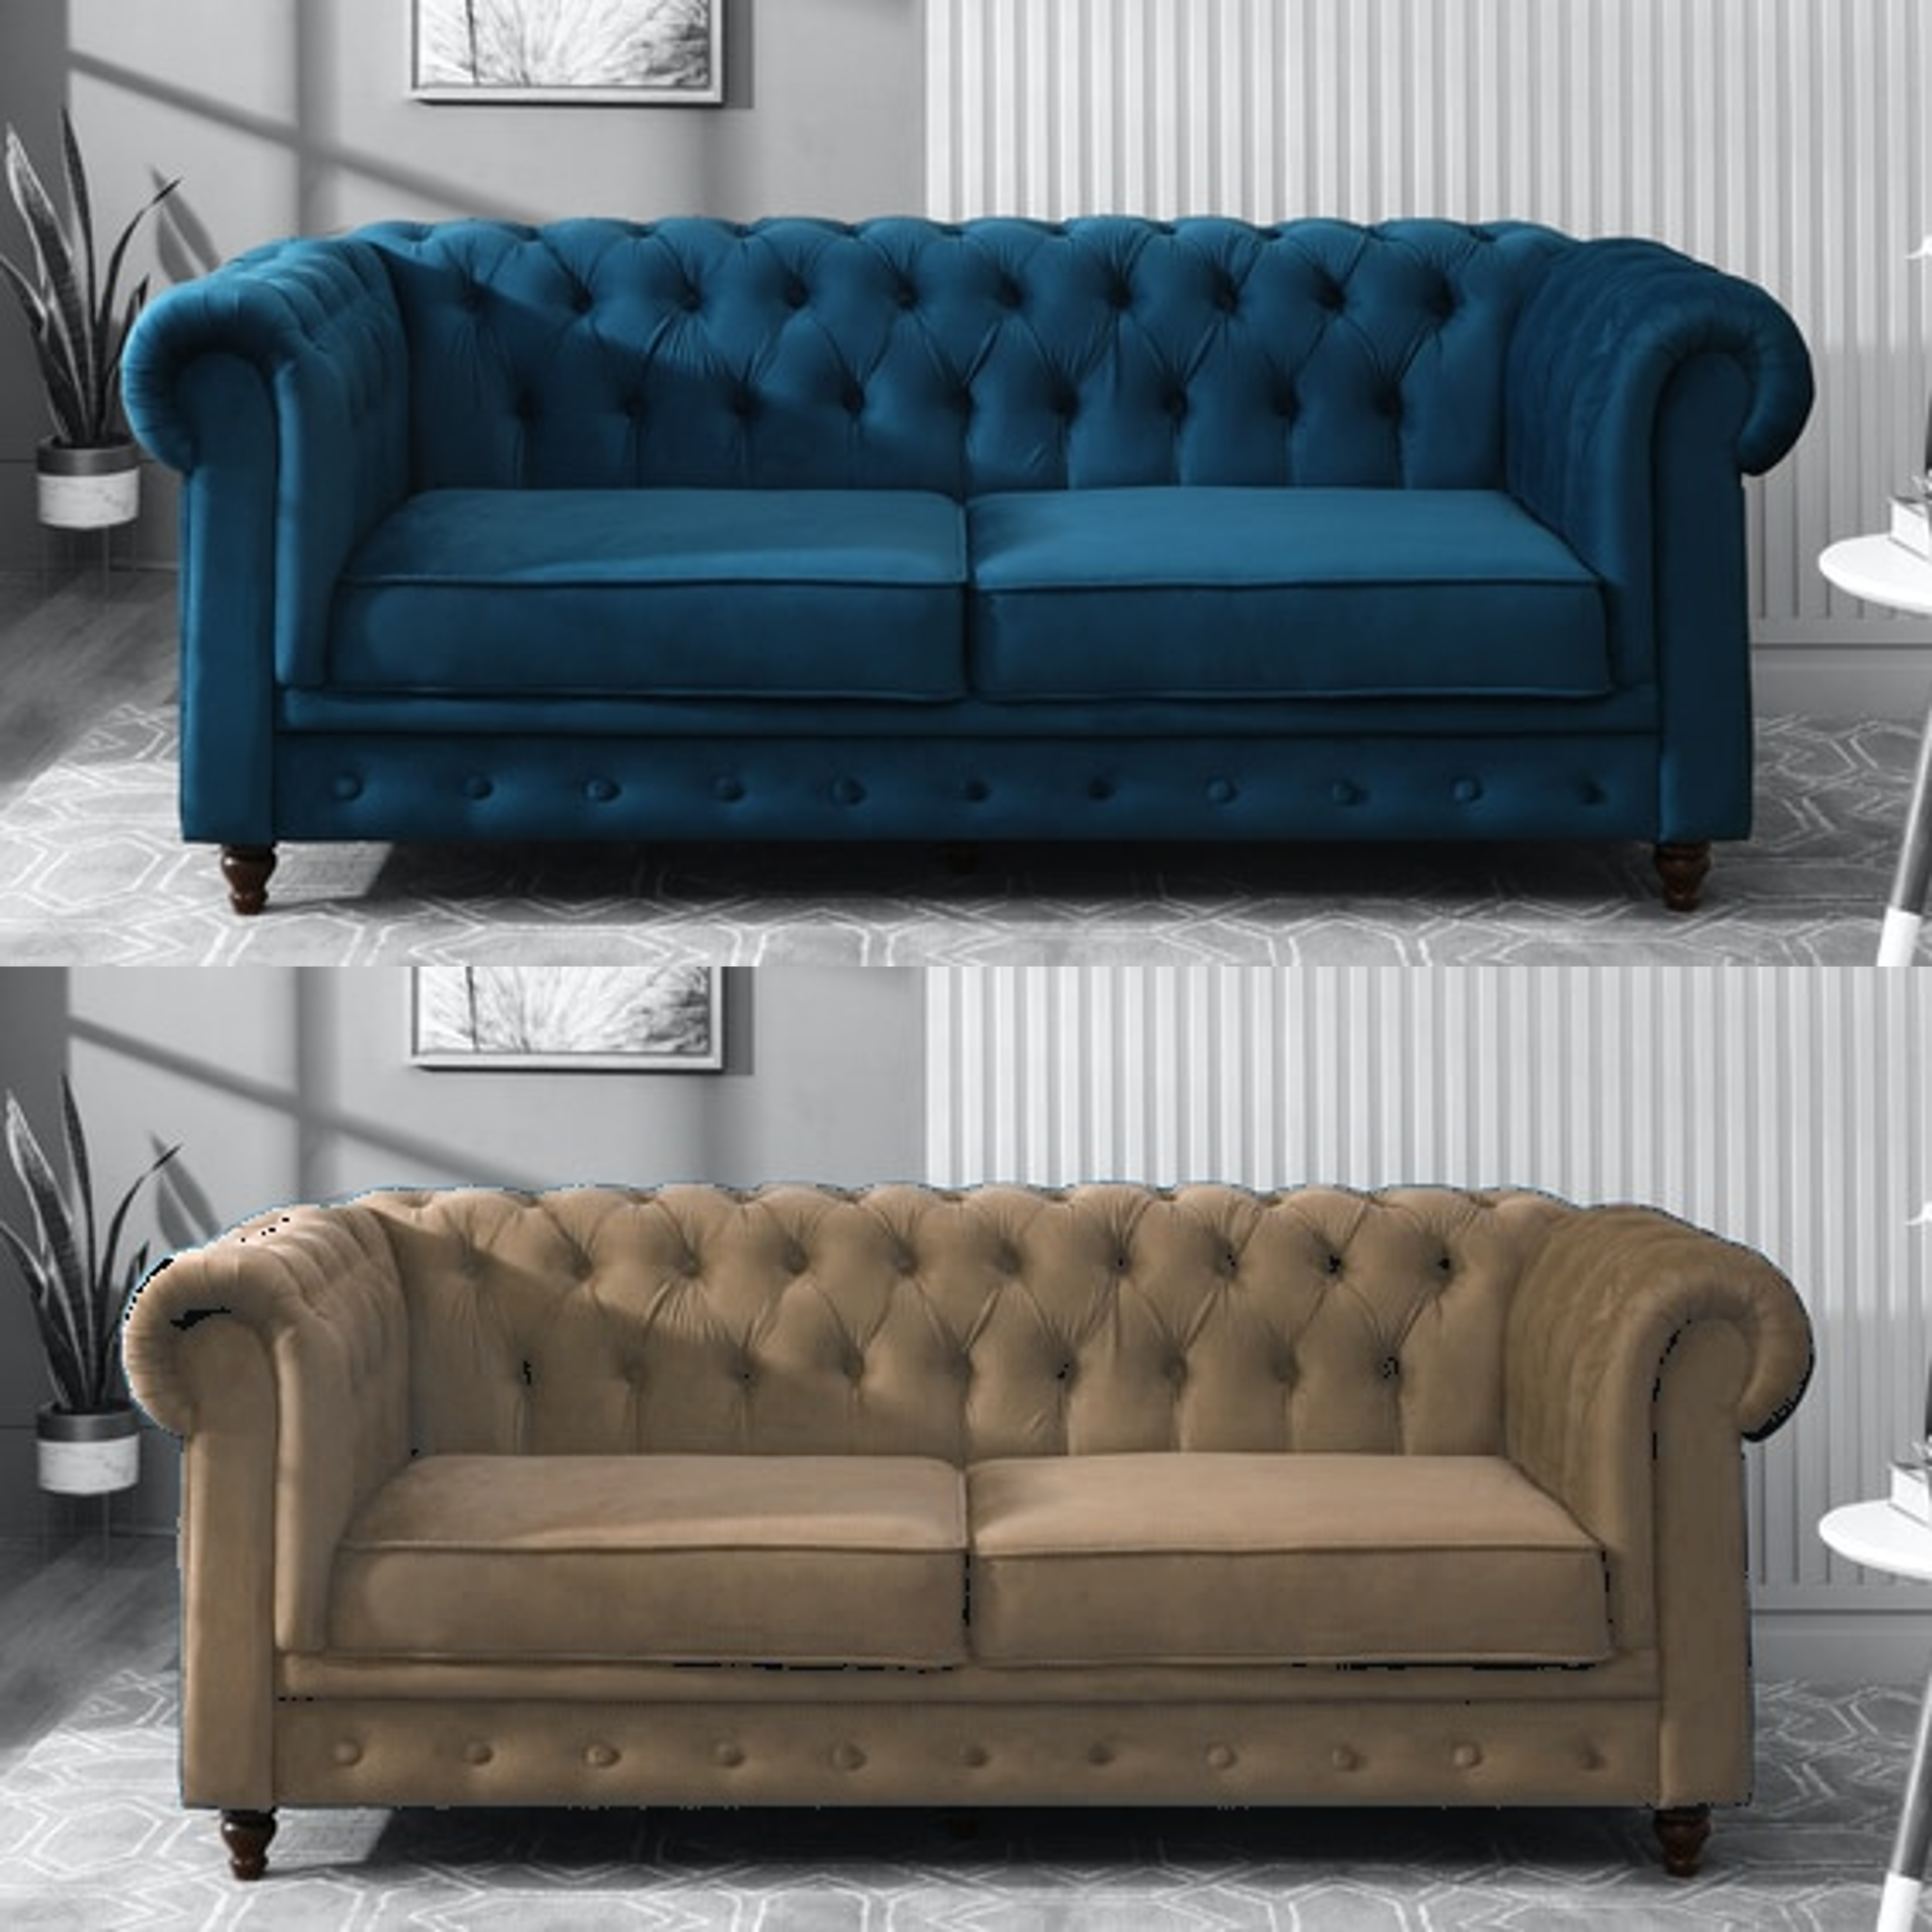
\includegraphics[width=0.5\linewidth]{Figures/boicanh2.png}
\end{figure}
Thay đổi màu của các đối tượng như đồ nội thất, trang phục, trang sức,...
\end{frame}

\begin{frame}{Phát biểu bài toán}
    \begin{table}
        \centering
        \begin{tabular}{ccc}
           \includegraphics[width=0.35\linewidth]{Figures/Picture1.png}  & \includegraphics[width=0.1\linewidth]{Figures/rightarrow.png} &  \includegraphics[width=0.35\linewidth]{Figures/2305_result.png} \\
           Ảnh xám ($I_g$) và điều kiện (c) & & Ảnh được tô màu ($I_{rgb}$)
        \end{tabular}
        \label{tab:my_label}
    \end{table}
    Vì đây là bài toán không đơn trị nên ta có thể mô hình hóa quá trình tô màu như một bài toán sinh mẫu từ một phân phối xác suất có điều kiện:
    \begin{equation*}
             I_{rgb} \sim P(I_{rgb}|I_g,c),
    \end{equation*}
    với c là điều kiện điều khiển quá trình tô màu (nếu có).
\end{frame}

\begin{frame}{Các thách thức của bài toán}

\begin{figure}
    \centering
    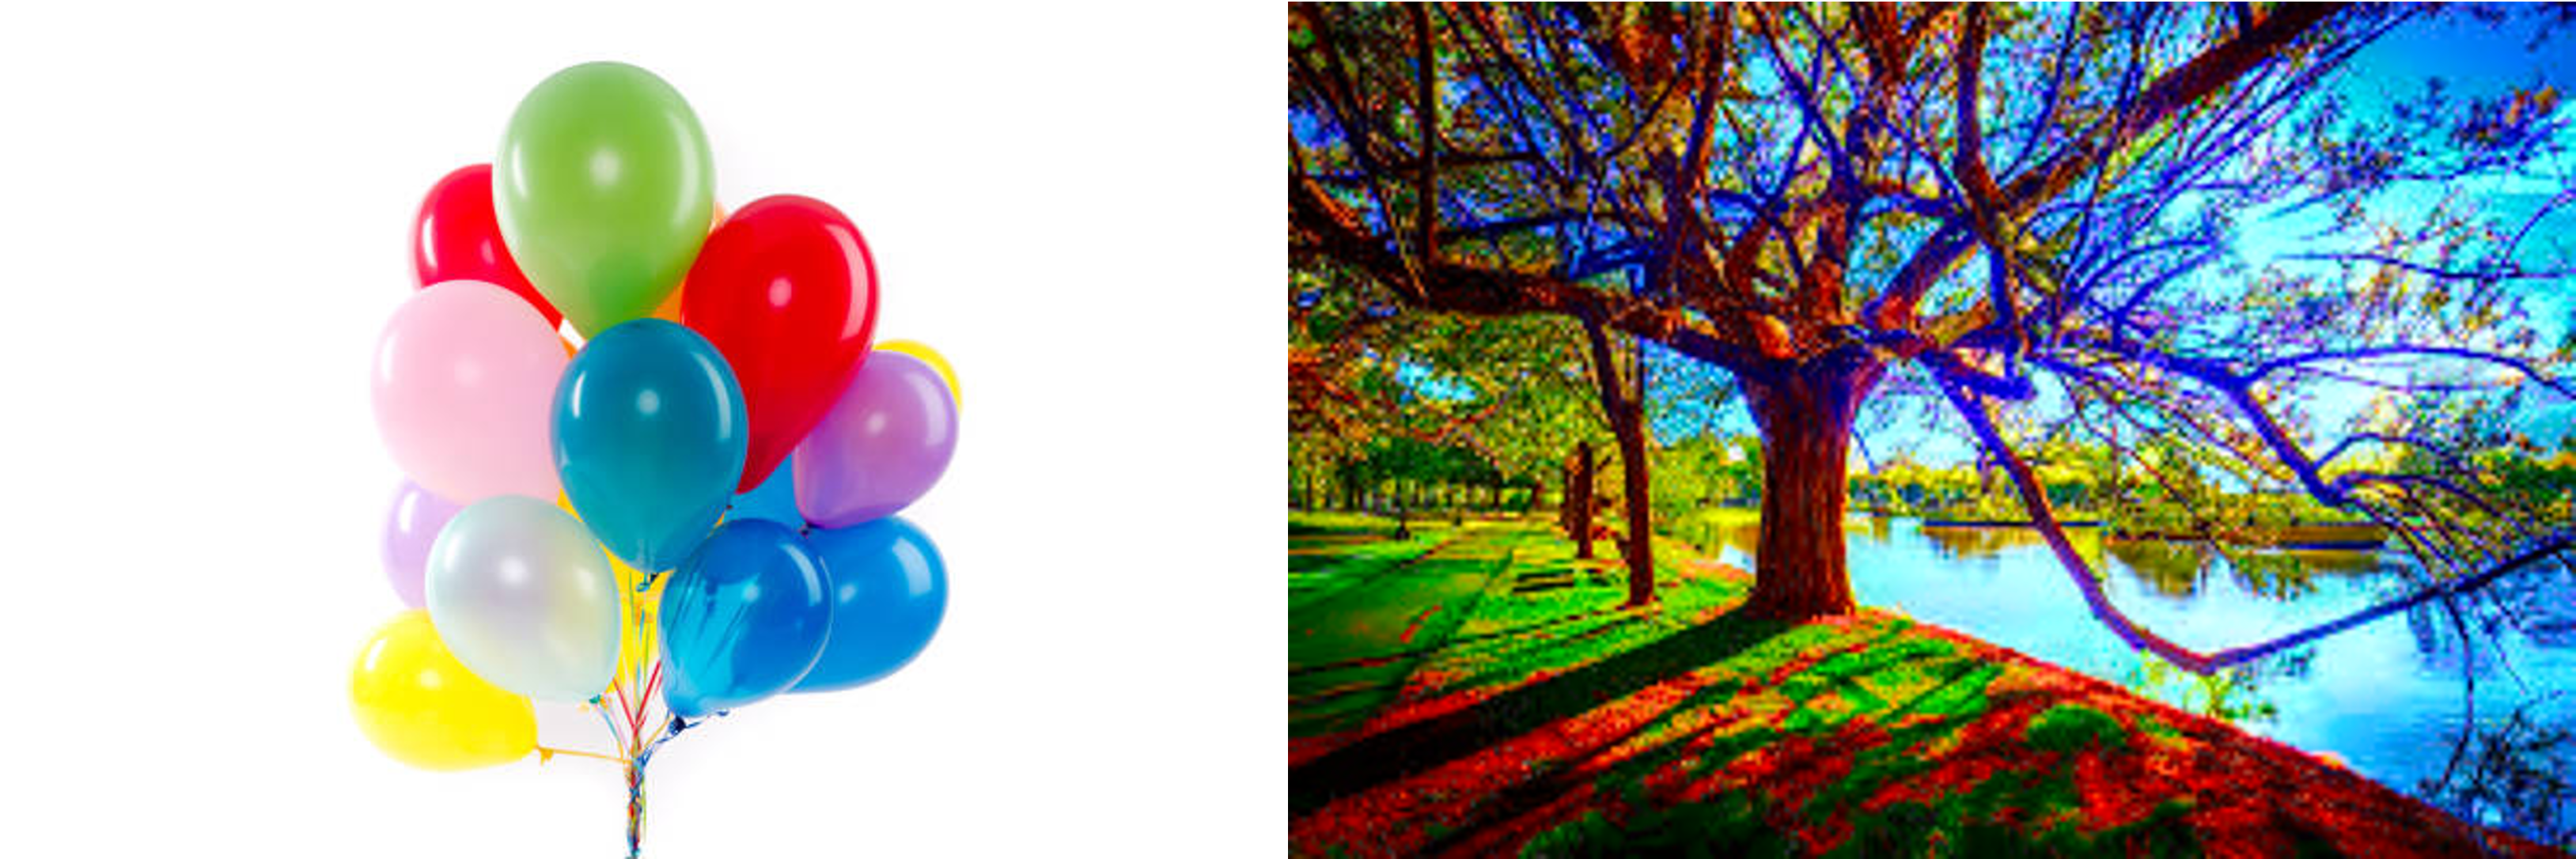
\includegraphics[width=0.8\linewidth]{Figures/hanche.png}
    \label{fig:enter-label}
\end{figure}

\begin{itemize}
    \item Đây là bài toán không đơn trị.

    \item Dễ gặp các lỗi lem màu, tô màu sai.

    \item Yêu cầu tương tác, tốn nhiều thời gian công sức.
\end{itemize}
    
\end{frame}

\begin{frame}{Mục tiêu}
    \begin{itemize}
        \item Xây dựng một mô hình tô màu ảnh độ xám đa phương thức dựa trên mô hình khuếch tán sao cho mô hình ít tiêu tốn tài nguyên trong quá trình huấn luyện và thực thi đồng thời cho ra ảnh màu có chất lượng tốt.
        \item Tìm hiểu sâu hơn về khả năng của các mô hình khuếch tán. Một mô hình đầy mạnh mẽ nhưng chưa được áp dụng quá nhiều vào lĩnh vực tô màu ảnh độ xám.
        \item Tạo ra các mô hình tô màu phục vụ cho các ứng dụng cụ thể.
        \item Tạo ra một giao diện đơn giản có thể giúp người dùng có thể dễ dàng sử dụng các mô hình được xây dựng.
    \end{itemize}
\end{frame}

